
\FloatBarrier
\section{General Concept}
\label{sec::61_gc}
To get started with and to understand the presented concepts that were implemented to generate dynamically balanced walking trajectories, one shall have a look at figure \ref{fig::61_pg}. The pattern generation therein (orange box), consists of four main building blocks: Forward kinematics, nonlinear model predictive control (NMPC), interpolation, and inverse kinematics, all of which were introduced in the theoretical foundations for humanoid walking section \ref{sec::2_hw}.
\begin{figure}[h!]
	\centering
	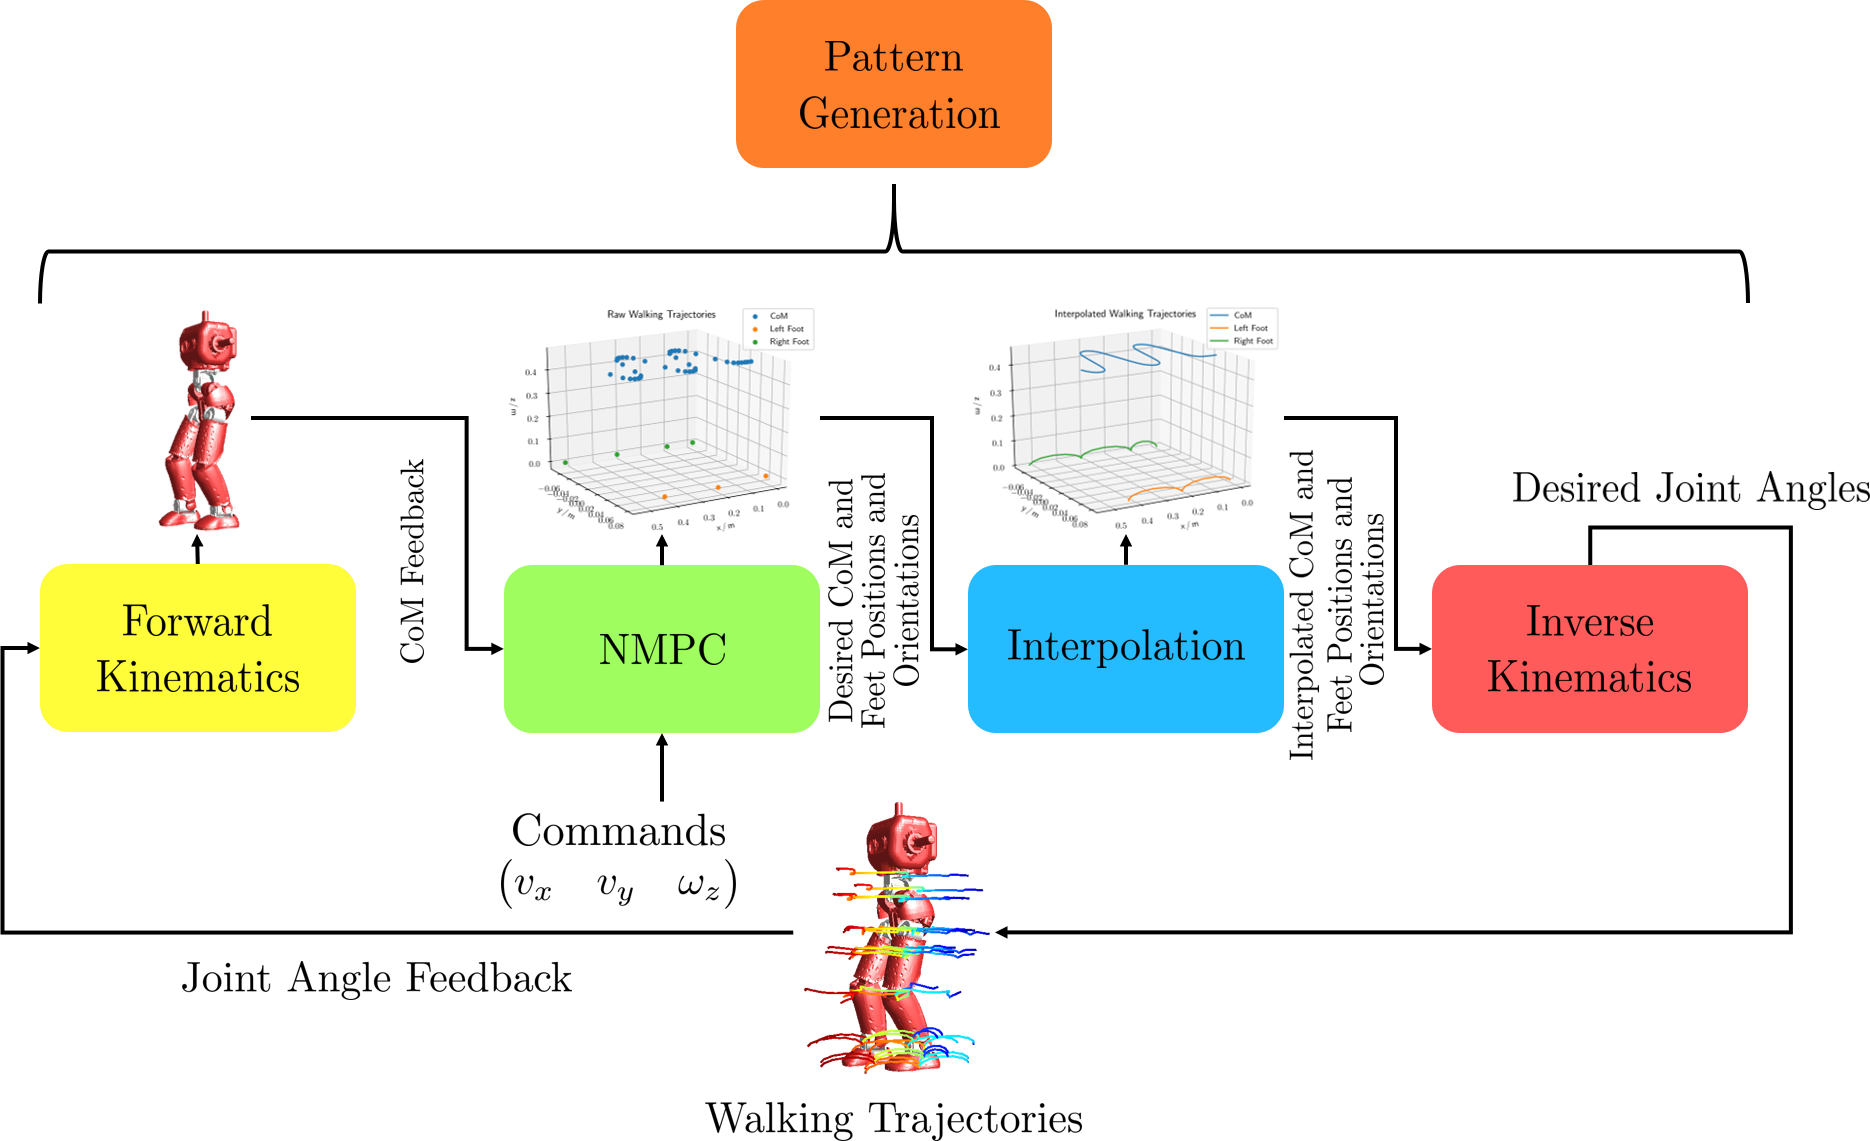
\includegraphics[scale=.5]{chapters/06_implementation_of_the_walking_pattern_generator/img/pattern_generation.png}
	\caption{Building blocks of the pattern generation that was implemented within the scope of this thesis.}
	\label{fig::61_pg}
\end{figure}
The natural entry point, to this otherwise closed control loop, is given by the commands that enter the nonlinear model predictive control. Commands are passed in the form of a desired velocity $\mathbf{v}_\text{ref}$ that the robot's center of mass (CoM) shall satisfy optimally according to the cost function that also takes dynamic balance and a smooth motion into account (equations \ref{eq::224_dcxy} to \ref{eq::224_dddcxy}). The future desired positions and orientations for the CoM, and the feet then result from the solution to the sequentially quadratic problem of equation \ref{eq::226_ocp} that tries to minimize this cost function. The balance criteria within this problem formulation bases upon the zero moment point (ZMP) around which the whole control framework builds. It is only by simplifying the robot's model that one can solve the optimal control problem in real-time. Therefore, one assumes the robot to be a linear inverted pendulum, for which, according to equations \ref{eq::211_zmp_x}, and \ref{eq::211_zmp_y}, a well-defined analytical relation between the CoM and the ZMP exists. The minimization of the distance between the analytical expression of the ZMP and the foot placement results in the desired dynamic balance. As shown in fig. \ref{fig::61_pg}, the desired CoM and the feet positions and orientation, as they are obtained from the NMPC, are sparsely distributed in space. Moreover, there is neither information about how the feet shall move along the z-axis, nor along the x-, and y-axis, but only where to place them in the x-y-plane. Therefore, as the subsequent step to the NMPC, one needs to add an interpolation. The interpolation interpolates the trajectories of the CoM via the linear time stepping scheme from section \ref{sec::232_ip} to obtain a finer sampling time. Additionally, the movement of the feet in the x-, y-, and z-direction, as well as their orientation, is computed by polynomials that are required to satisfy the initial and end conditions of the foot placement. These polynomials are expressed in terms of equations \ref{eq::231_pos_poly} to \ref{eq::231_acc_poly}, and they are set to be of 5th order for the x-, and the y-positions of the feet, as well as for the orientations, where the coefficients $a_i$ are computed according to equation \ref{eq::231_ai_5th}. The z-positions, on the other hand, are computed via 4th order polynomials with coefficients from equation \ref{eq::231_ai_4th}. Put together, the nonlinear model predictive control and the interpolation between the resulting subsequent solutions for the positions and orientation of both, the CoM and the feet, describe dynamically balanced trajectories, given that the humanoid robot of interest resembles the physics of an inverted pendulum. Now to bridge the gap between dynamically balanced trajectories in Cartesian space, and a humanoid robot that satisfies them with its CoM and its feet, the inverse kinematics problem needs to be addressed. The inverse kinematics, which follow immediately after the interpolation step, take the positions and orientations of the CoM and the feet as constraints and find a composite of joint angles that fulfill them. The inverse kinematics within this work is computed via the Rigid Body Dynamics Library (RBDL) \cite{felis2017rbdl}. The continuity of subsequent solutions is therein assured by initializing the inverse kinematics with the previous solution. Resulting joint angles, once passed to the humanoid, then result in walking trajectories, as indicated in fig. \ref{fig::61_pg} by the colored lines at the joints of the robot. Due to the inherent mismatch of the robot's physics from that of an inverted pendulum, as well as other effects like friction, there is a chance that the desired joint angles differ from the achieved ones. To compensate for the discrepancy, the last building block of the pattern generation is the feedback of the measured CoM to the NMPC. The CoM, therein, is computed by reading out the achieved joint angles, so that the forward kinematics from RBDL can be utilized to determine the positions and orientations of the humanoid's links in space, and therefore the true CoM.





 